
\section{Setting a Baseline}
\subsection{Required submission files}
\begin{enumerate}
	\item \hl{The updated gauss.c.}
	
	\verb!/Collective/gauss.c!

	\item \hl{The performance plots and description in the report.}
		
	Performance plots are seen in Figs. \ref{fig:total_multdomain_collective_baseline}, \ref{fig:total_multprocess_collective_baseline}, \ref{fig:mpi_multdomain_collective_baseline},
	\ref{fig:mpi_multprocess_collective_baseline}, \ref{fig:compute_multdomain_collective_baseline},
	\ref{fig:compute_multprocess_collective_baseline}, \ref{fig:vampir_baseline} and \ref{fig:vampir_collective}.

\end{enumerate}

\subsection{Questions}
\begin{enumerate}
	\item \hl{Which patterns were identified and replaced with collective communication in the code? Explain.}
	
	There were several regions that could be replaced with collective communication:
	\begin{enumerate}
	\item The fan-out when data is sent from the root process to all other processes. This could be replaced by a simple \verb!MPI_Bcast! operation. 
	
	\item The sending of pivot entries to each other process after performing the elimination and normalization step. The sending and the calculation steps were done completely sequentially---the process with the current pivot entry would finish the gaussian ellimination steps on the entire local block before any sending took place. We interleaved \verb!MPI_Ibcast! collective operations such that each row would be sent to each other process via a non-blocking collective broadcast once computation on it was complete.
	
	\item The sending of segments of the processed solution vector to perform a "triangular solve". We used a series of \verb!MPI_Bcast! operations to send this information instead of \verb!MPI_Send! operations in for loops
	
	\item The fan-in of the solution vector to the root process. We used an \verb!MPI_Gather! to collect the solution vector into the \verb!solution! array.
	
	\end{enumerate}
	
	\item \hl{Were you able to identify any potential for overlap and used any non-blocking collectives? (Use Vampir)}	
	
	Theoretical overlap can be achieved during the sending of rows during the computation steps. 
	We implemented the non-blocking collective \verb!MPI_Ibcast! once each row was ready to be sent. 
	Each other process would start the corresponding \verb!MPI_Ibcast! operation for 
	all rows from the process with the pivot row; an \verb!MPI_Wait! function would be 
	called before the exact pivot line was used for calculation.
	
	This would result in calculation/communication overlap, as new rows 
	would be received as calculation using previous rows was taking place. 
	We can compare the Vampir plots to see the difference between blocking
	and non-blocking communication, in Fig. \ref{fig:vampir_collective}. and
	 \ref{fig:vampir_baseline}
	
	\begin{figure}[h] % h=here, t=top, b=bottom, p=(extra)page, !=force
		\centering
		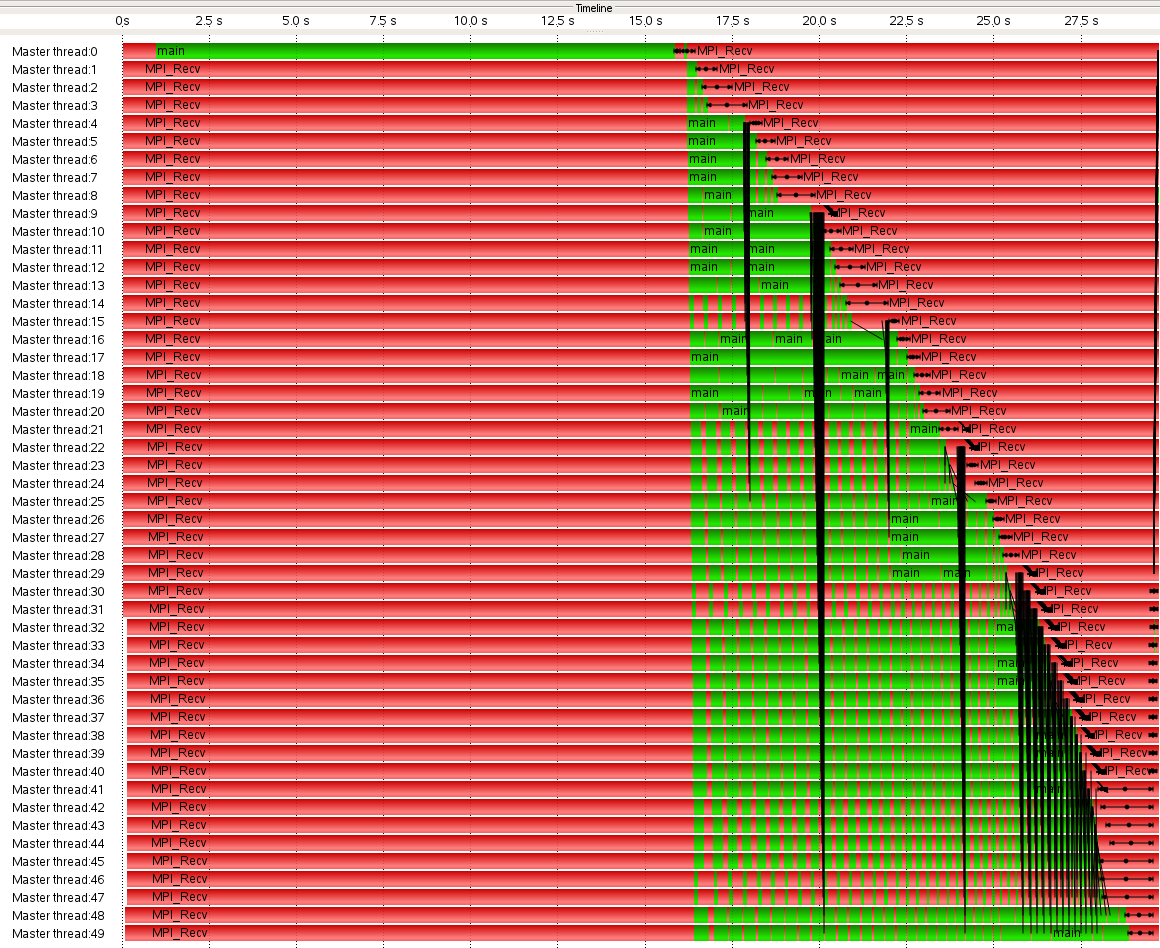
\includegraphics[width=.8\linewidth]{baseline/baseline_vampir_biggest_size_timeline.png}
		\caption{Vampir Output for Baseline Implementation}
		\label{fig:vampir_baseline}
	\end{figure}	
	
	\begin{figure}[h] % h=here, t=top, b=bottom, p=(extra)page, !=force
		\centering
		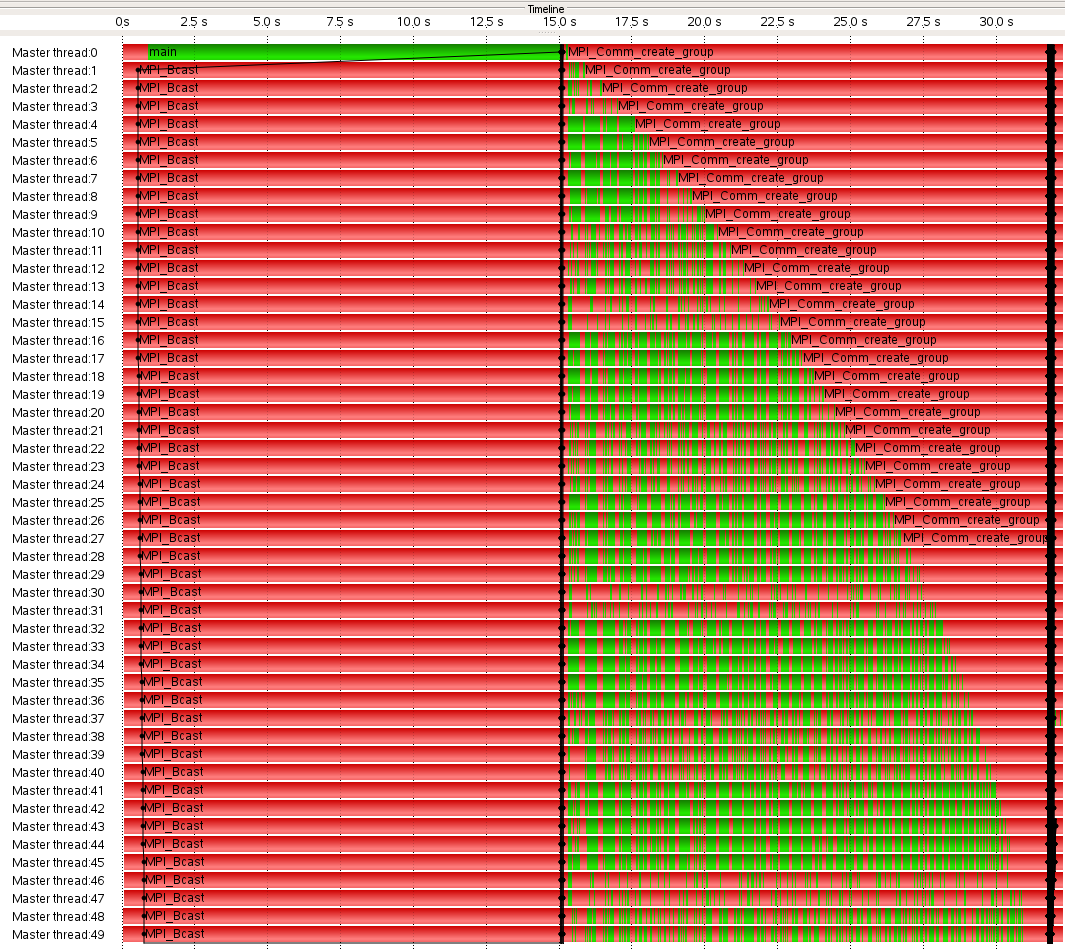
\includegraphics[width=.8\linewidth]{collective/collective_vampir_biggest_size_timeline.png}
		\caption{Vampir Output for Collective Implementation}
		\label{fig:vampir_collective}
	\end{figure}	
	
	There was overlap achieved when implementing this function. We know that if no overlap occured,
	we should be able to see the repeated waits from the broadcast functions present throughout
	the computation segments. However, when looking closely at the code, the waits are very small
	in size and not present in certain regions. This indicates that computation and communication did
	take place.
	
	\item \hl{Was there any measurable performance or scalability improvement as a result of these changes?}		
	
	We changed both the communication scheme and the computation process when updating to use
    collective operations. Thus, we have to examine total time, MPI time and compute times for
    the new implementation. 
    
    We see from the total time, in Fig. \ref{fig:total_multdomain_collective_baseline} and
    \ref{fig:total_multprocess_collective_baseline},
     that there is not actually a large amount of time savings as a result
    of these changes. We do see that the updated program does, for the certain set of parameters,
    outperform the baseline version.
    
    Specifically, we see that the collective communication implementation is slightly faster
    once the size of the domain is increased beyond a certain limit. This is not unexpected
    as we asnychronously communicate each line once it is modified by the GE algorithm
    ---allowing for communication and computation overlap. The benefit of this overlap should
    be more pronounced when each process needs to compute larger domain sizes.
    
	\begin{figure}[h] % h=here, t=top, b=bottom, p=(extra)page, !=force
		\centering
		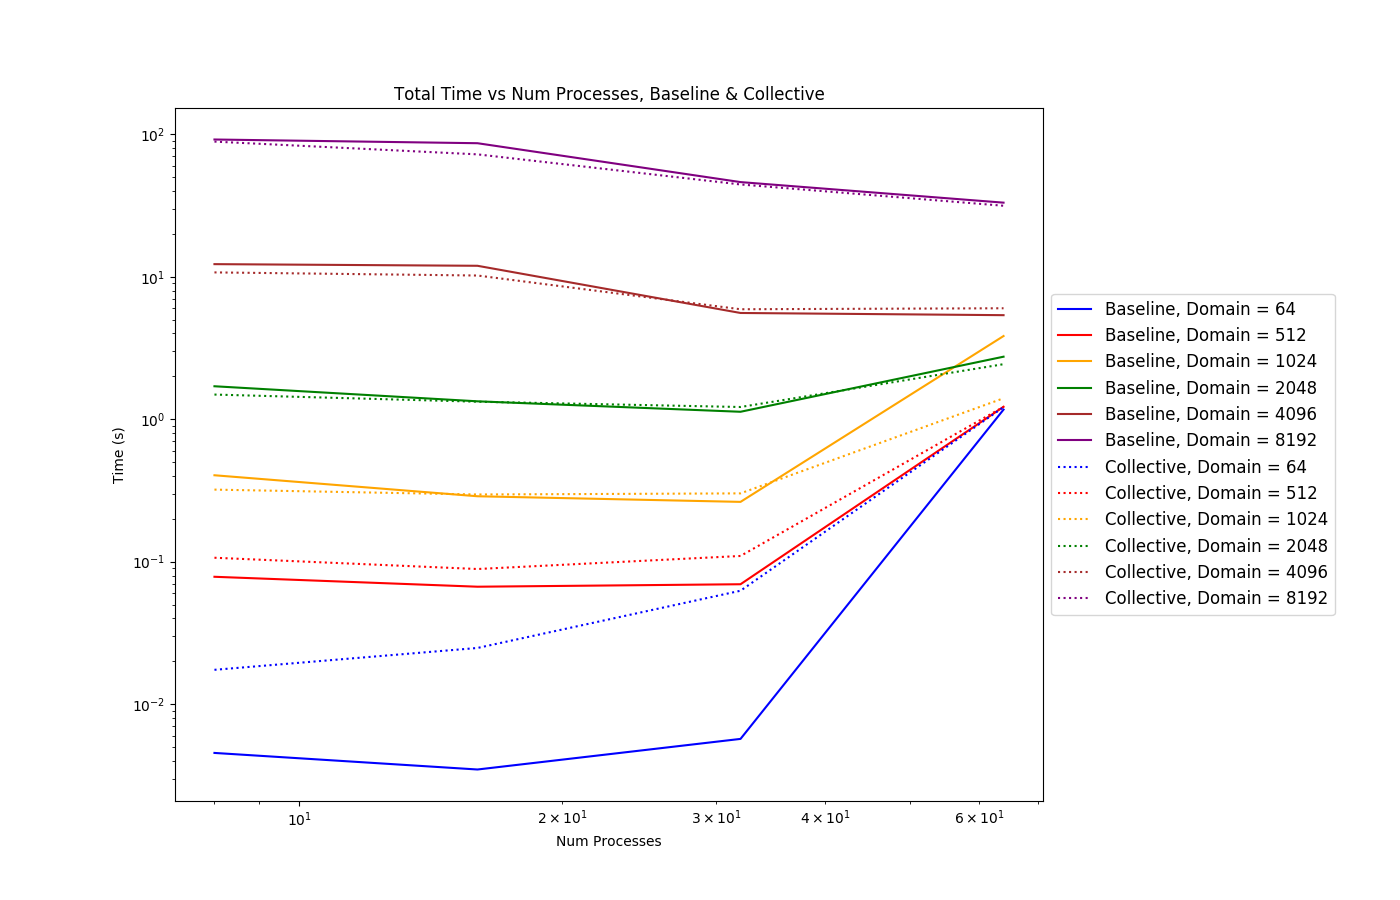
\includegraphics[width=.8\linewidth]{collective/total_multdomain_haswell_collective_baseline.png}
		\caption{Total Time vs. \#Processes., Collective vs. Baseline}
		\label{fig:total_multdomain_collective_baseline}
	\end{figure}	
	
	\begin{figure}[h] % h=here, t=top, b=bottom, p=(extra)page, !=force
		\centering
		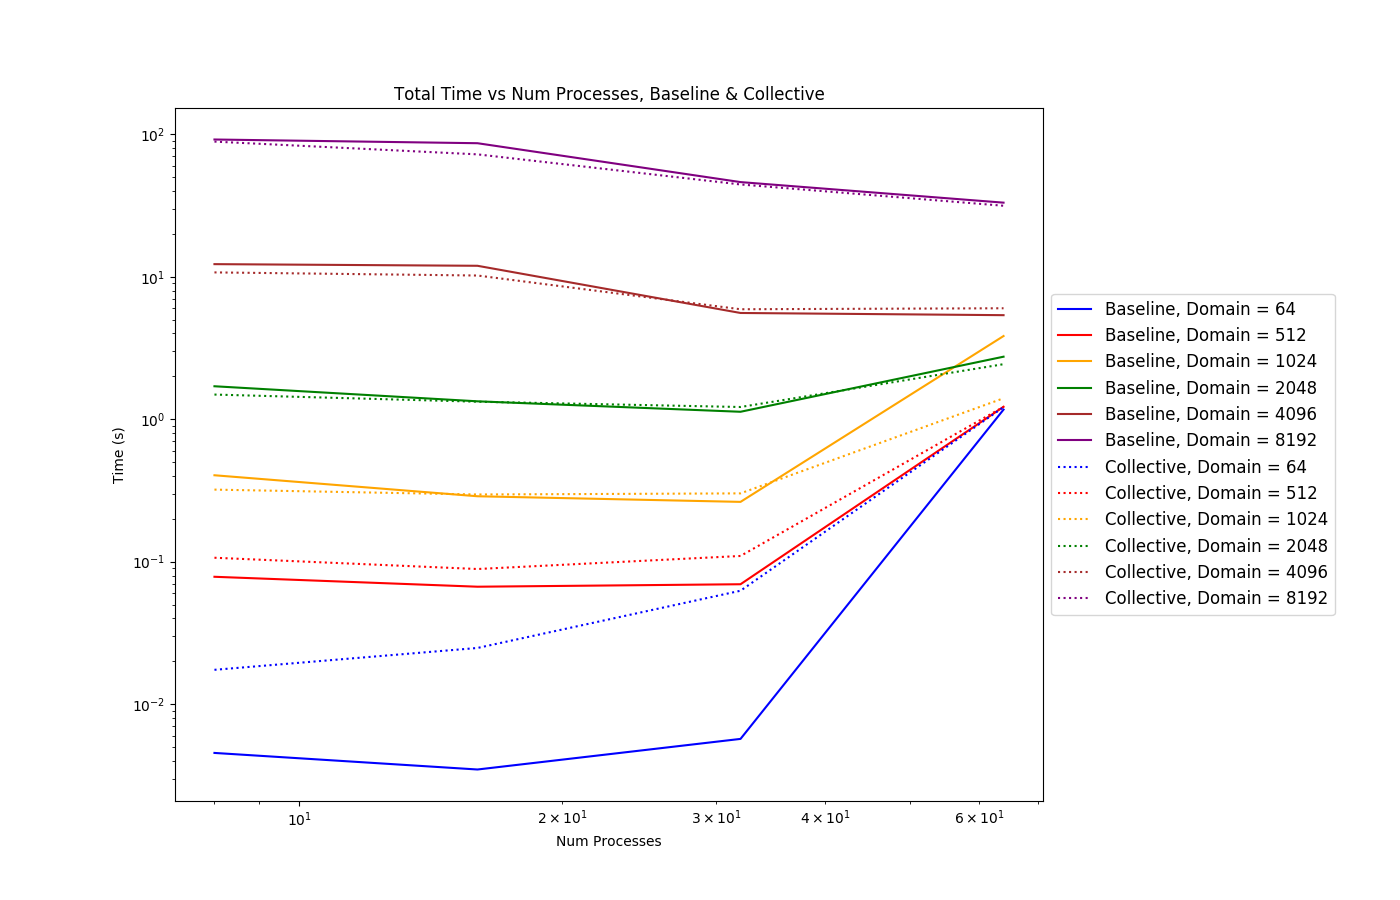
\includegraphics[width=.8\linewidth]{collective/total_multdomain_haswell_collective_baseline.png}
		\caption{Total Time vs. Domain Size., Collective vs. Baseline}
		\label{fig:total_multprocess_collective_baseline}
	\end{figure}	
    
    We do have somewhat interesting results for the MPI time and the compute time.
    Firslty, the MPI time can be seen in Fig. \ref{fig:mpi_multdomain_collective_baseline} and
	\ref{fig:compute_multprocess_collective_baseline}. These two figures show a very impressive
	drop in the MPI time when implementing non-blocking collective calls. Now that we are able
	to continue computation during communication, it is expected that the amount of time spend
	waiting for communication or wait calls is very short.
	
	\begin{figure}[h] % h=here, t=top, b=bottom, p=(extra)page, !=force
		\centering
		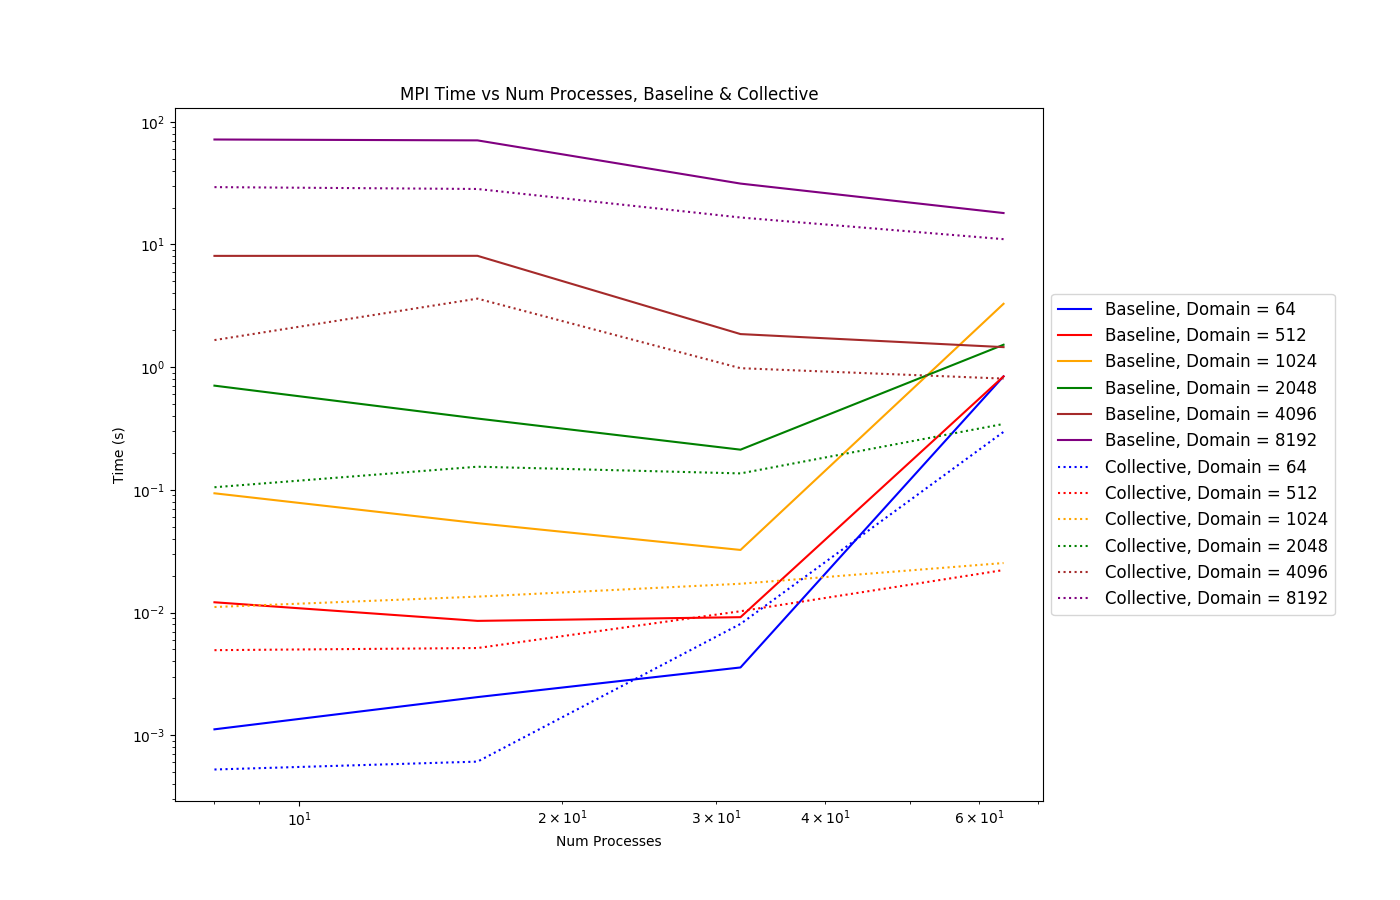
\includegraphics[width=.8\linewidth]{collective/mpi_multdomain_haswell_collective_baseline.png}
		\caption{MPI Time vs. \#Processes., Collective vs. Baseline}
		\label{fig:mpi_multdomain_collective_baseline}
	\end{figure}	
	
	\begin{figure}[h] % h=here, t=top, b=bottom, p=(extra)page, !=force
		\centering
		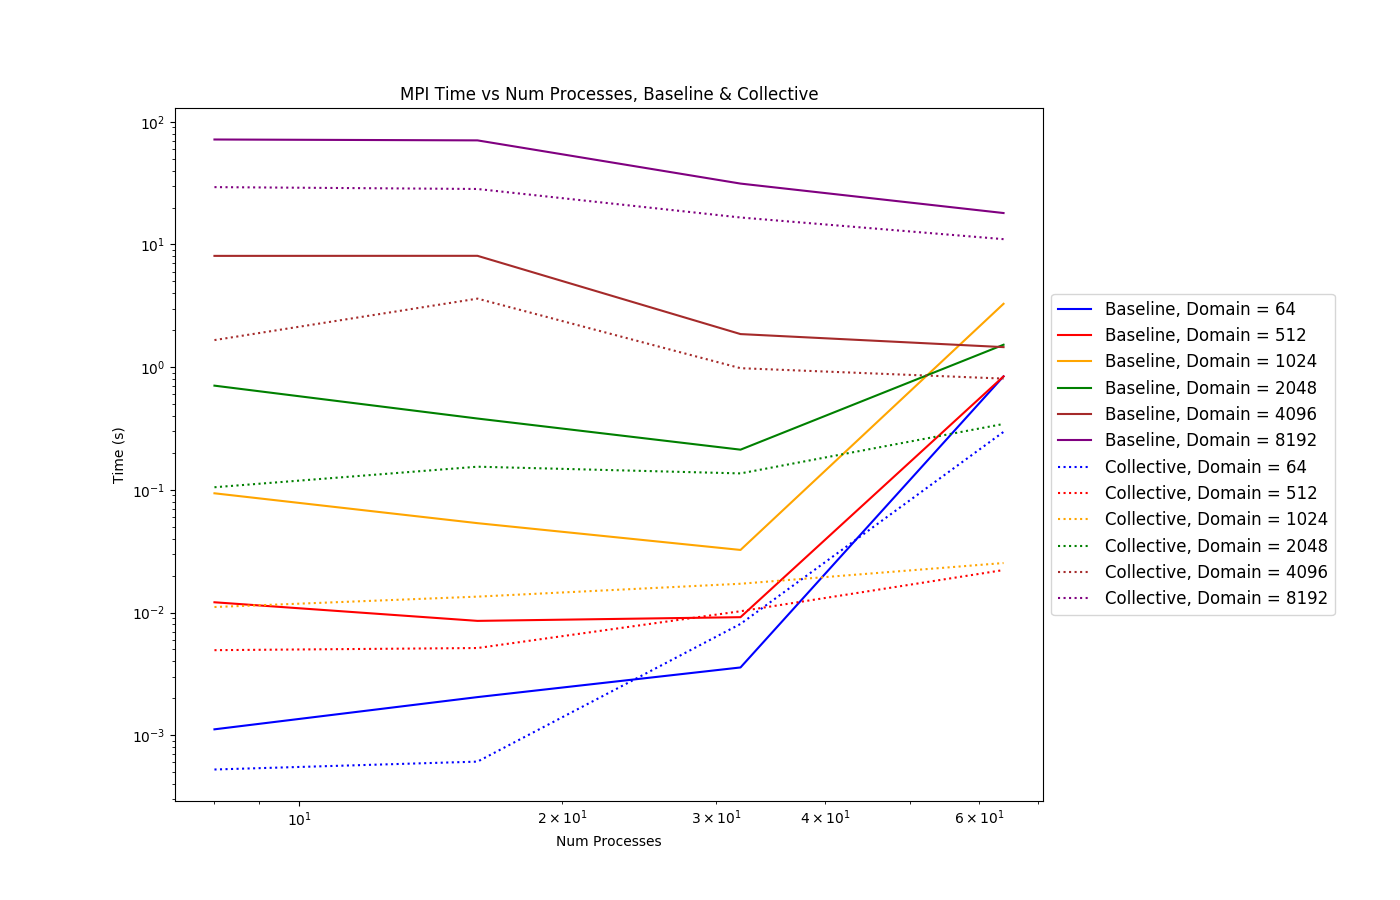
\includegraphics[width=.8\linewidth]{collective/mpi_multdomain_haswell_collective_baseline.png}
		\caption{MPI Time vs. Domain Size., Collective vs. Baseline}
		\label{fig:mpi_multprocess_collective_baseline}
	\end{figure}	
	
 	However, we do see that there is an increase in compute time 
 	overall---shown in Fig. \ref{fig:compute_multdomain_collective_baseline} and
	\ref{fig:compute_multprocess_collective_baseline}. We expected this, to some extent, as we now load a new 
	line into a send buffer (or unload a new line from a receive buffer) each time it is ready. However,
	this does not fully explain why our compute time is significantly slower.
	
	Further testing from our end indicated that the repeated creation and definition of \verb!MPI_Comm!s and
	\verb!MPI_Group!s for the repeated broadcasts which were taking up extremely long periods of time. We did
	not initially detect this as we only recorded the time required for communication or wait calls to return.
	This phenomenon explained why compute times were so long even for very small sample sizes---the overhead
	for creating additional communication channels and groups was dependent on the number of processes. 

		\begin{figure}[h] % h=here, t=top, b=bottom, p=(extra)page, !=force
		\centering
		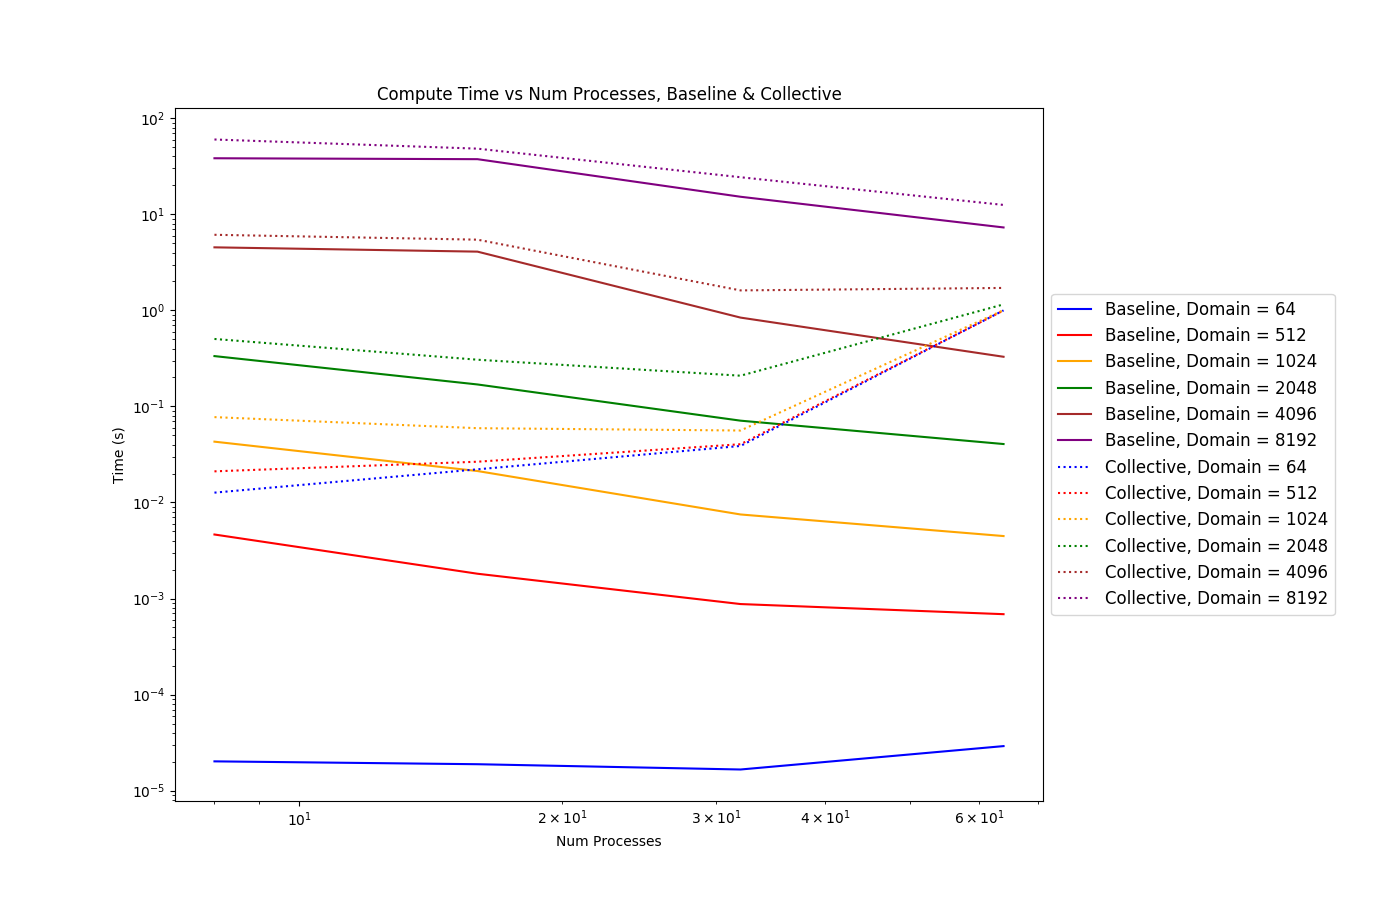
\includegraphics[width=.8\linewidth]{collective/compute_multdomain_haswell_collective_baseline.png}
		\caption{Compute Time vs. \#Processes., Collective vs. Baseline}
		\label{fig:compute_multdomain_collective_baseline}
	\end{figure}	
	
	\begin{figure}[h] % h=here, t=top, b=bottom, p=(extra)page, !=force
		\centering
		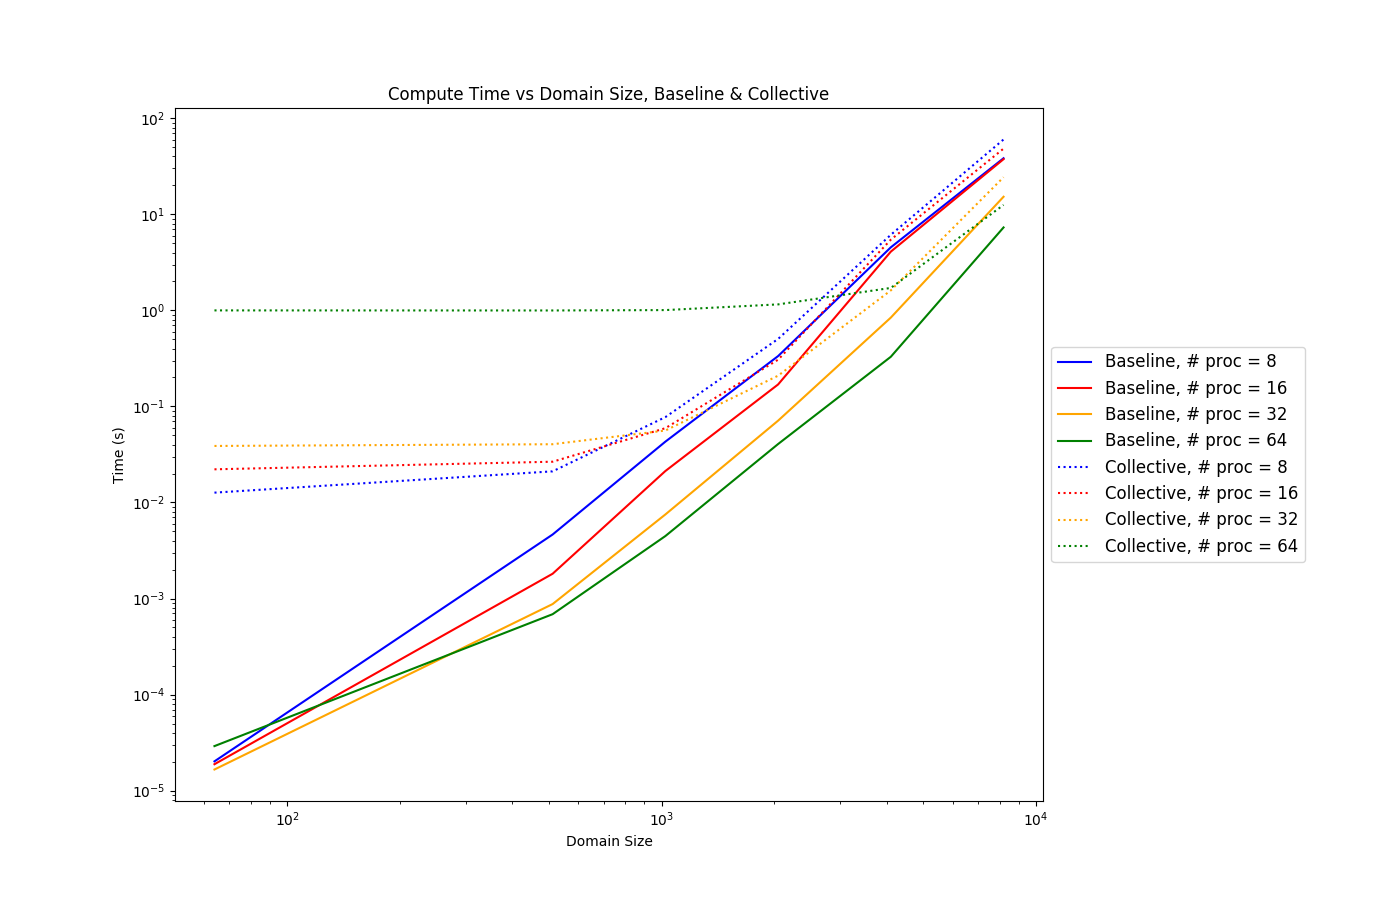
\includegraphics[width=.8\linewidth]{collective/compute_multproc_haswell_collective_baseline.png}
		\caption{Compute Time vs. Domain Size., Collective vs. Baseline}
		\label{fig:compute_multprocess_collective_baseline}
	\end{figure}	
	
	Thus, in order to resolve this situation, we need to investigate cheaper ways to set up communication
	and groups in the MPI. If we resolve this, the scaling improvement due to the use of collective 
	operations will become more obvious.
	
	\item \hl{Is the resulting code easier to understand and maintain after the changes? Why?}	
	
	Certain segments of the code are easier to understand, while certain segments of the code are more 		
	complicated. We have replaced large for loops with collective operations---this reduces 
	\verb!MPI_Send!/\verb!MPI_Recv! calls with a single collective call. The code is then less dense and it
	 is easier to see how data is distributed among the various process ranks.

	However, we also employ custom \verb!MPI_Group!s/\verb!MPI_Comm!s to control the sets of 
	processes that are involved in each collective operation. This is a more advanced use of MPI 
	functions and basic users may be confused. 

	Overall, the code is easier to maintain, in the sense that the individual chunks are easier to 
	read. However, the cost of collective operations is the lack of flexibility---adapting the code 
	for additional functionality or for greater generality will be harder as we have replaced all p2p 
	communications with collective operations, ie. this may need to be reverted if the algorithm is 
	changed.	
	
\end{enumerate}

		


% % Figure example
% \begin{figure}[p] % h=here, t=top, b=bottom, p=(extra)page, !=force
%  	\begin{center}
%  		
\includegraphics[width=.9\linewidth]{figure.png} % It searches in the Figures/ folder!
%  		\caption{Caption text}
%  		\label{fig:figureLabelName}
%  	\end{center}
% \end{figure}
